\documentclass[11pt,a4paper]{article}

\usepackage[utf8]{inputenc}
\usepackage{amsmath, amssymb, amsfonts}
\usepackage{graphicx}
\usepackage{tikz}
\usetikzlibrary{positioning} % <-- important for node positioning
\usepackage{hyperref}
\usepackage{geometry}
\usepackage{caption}
\geometry{margin=2.5cm}

\title{Conditional Variational Autoencoder (CVAE) for Single-Cell RNA-seq Data}
\author{Tutorial Documentation}
\date{}

\begin{document}

\maketitle

\section{Motivation and Biological Background}

Single-cell RNA sequencing (scRNA-seq) enables the quantification of gene expression at the level of individual cells. Each cell is represented by a count vector
\[
x_i = [x_{i1}, x_{i2}, \ldots, x_{iG}],
\]
where $x_{ij}$ denotes the number of mRNA transcripts for gene $j$ in cell $i$. The resulting data matrix $X \in \mathbb{N}^{N \times G}$ is high-dimensional, sparse, and overdispersed.

In practice, cells are processed in separate \emph{experimental batches}, corresponding to different sequencing runs, tissue donors, or laboratories. These batches introduce \textbf{technical variability} unrelated to biological differences between cells. Such unwanted sources of variation are known as \textbf{batch effects}. If not corrected, batch effects can confound analyses, leading to clusters that reflect experimental artifacts rather than true biological distinctions.

To address this issue, we use a \textbf{Conditional Variational Autoencoder (CVAE)}. This probabilistic model learns a latent representation $Z$ that captures biological variation while explicitly conditioning on batch information $B$, allowing it to model and correct for technical effects.

\section{Model Overview}

The CVAE defines a probabilistic model for the observed data $X$, the latent variables $Z$, the batch covariates $B$, and optionally the cell class labels $C$:
\[
p(X, C, Z \mid B) = p(Z)\,p(C \mid Z)\,p(X \mid Z, B),
\]
where
\begin{itemize}
  \item $Z$ represents the latent biological state of a cell,
  \item $B$ encodes known experimental batch covariates,
  \item $C$ represents an optional cell-type or class label, and
  \item $X$ are observed gene expression counts.
\end{itemize}

The corresponding generative process is summarized as:
\[
Z, B \rightarrow X, \qquad Z \rightarrow C.
\]

\subsection*{Graphical Model}

\begin{figure}[h!]
\centering
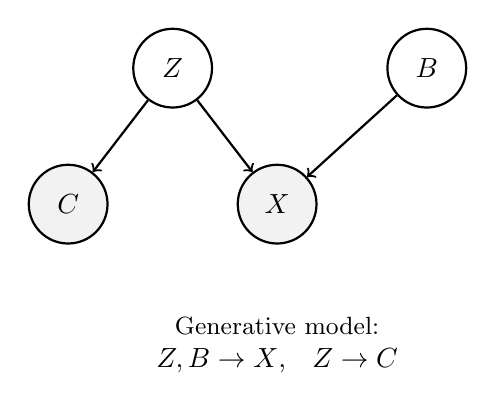
\begin{tikzpicture}[
  node distance=2.5cm,
  latent/.style={circle, draw=black, thick, minimum size=1cm},
  obs/.style={circle, draw=black, thick, fill=gray!10, minimum size=1cm},
  arrow/.style={->, thick}
]

\node[latent] (z) {$Z$};
\node[latent, right=2.2cm of z] (b) {$B$};
\node[obs, below right=1cm and 0.6cm of z] (x) {$X$};
\node[obs, below left=1cm and 0.6cm of z] (c) {$C$};

\draw[arrow] (z) -- (x);
\draw[arrow] (b) -- (x);
\draw[arrow] (z) -- (c);

\node[below=0.8cm of x, align=center] {\small Generative model: \\ $Z,B \to X$, \; $Z \to C$};

\end{tikzpicture}
\caption{Graphical model of the Conditional Variational Autoencoder (CVAE).}
\end{figure}

The decoder $p_\theta(X \mid Z, B)$ models the gene expression counts given the latent biological representation and batch effects. The model assumes a Negative Binomial likelihood, appropriate for overdispersed count data:
\[
X_{ij} \sim \mathrm{NB}(\mu_{ij}, \theta_{ij}),
\]
where $\mu_{ij}$ is the predicted mean expression and $\theta_{ij}$ is a gene-specific dispersion parameter.

\section{Inference Model}

Direct computation of the posterior $p(Z \mid X, B)$ is intractable. Therefore, we approximate it with an encoder network
\[
q_\phi(Z \mid X, B) = \mathcal{N}\!\big(\mu_\phi(X, B), \mathrm{diag}(\sigma_\phi^2(X, B))\big),
\]
which predicts the mean and variance of a Gaussian distribution. Samples from this approximate posterior are obtained via the \textbf{reparameterization trick}:
\[
Z = \mu_\phi(X, B) + \sigma_\phi(X, B) \odot \epsilon, \quad \epsilon \sim \mathcal{N}(0, I),
\]
allowing gradients to flow through stochastic nodes during optimization.

\begin{figure}[h!]
\centering
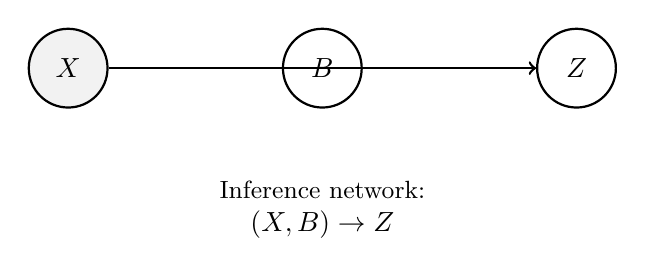
\begin{tikzpicture}[
  node distance=2.8cm,
  latent/.style={circle, draw=black, thick, minimum size=1cm},
  obs/.style={circle, draw=black, thick, fill=gray!10, minimum size=1cm},
  arrow/.style={->, thick}
]

\node[obs] (x) {$X$};
\node[latent, right=2.2cm of x] (b) {$B$};
\node[latent, right=2.2cm of b] (z) {$Z$};

\draw[arrow] (x) -- (z);
\draw[arrow] (b) -- (z);

\node[below=0.8cm of b, align=center] {\small Inference network: \\ $(X,B) \to Z$};

\end{tikzpicture}
\caption{Inference model (encoder) used to approximate $p(Z \mid X,B)$.}
\end{figure}

\section{Training Objective: Evidence Lower Bound (ELBO)}

We aim to maximize the log-likelihood $\log p(X \mid B)$, which involves an intractable integral over the latent variable $Z$:
\[
\log p(X \mid B) = \log \int p(X, Z \mid B) \, dZ.
\]

By introducing the approximate posterior $q_\phi(Z \mid X, B)$ and applying Jensen's inequality, we obtain the \textbf{Evidence Lower Bound (ELBO)}:
\[
\mathcal{L}_{\text{ELBO}} =
\mathbb{E}_{q_\phi(Z \mid X, B)}[\log p_\theta(X \mid Z, B) + \log p_\theta(C \mid Z)]
- \mathrm{KL}\big(q_\phi(Z \mid X, B) \, \| \, p(Z)\big).
\]

\noindent
The terms correspond to:
\begin{itemize}
  \item A \textbf{reconstruction term}, encouraging accurate modeling of the observed data;
  \item An optional \textbf{classification term}, encouraging correct prediction of cell classes;
  \item A \textbf{KL divergence term}, regularizing the approximate posterior to remain close to the prior $p(Z) = \mathcal{N}(0, I)$.
\end{itemize}

The model is trained by maximizing this ELBO using stochastic gradient ascent. Sampling of $Z$ is handled via the reparameterization trick, and gradients are estimated efficiently through automatic differentiation. In practice, this is implemented using the \texttt{pyro} probabilistic programming framework, which provides stochastic variational inference (SVI).

\section{Model Architecture}

The neural components of the CVAE are implemented using standard PyTorch modules:
\begin{itemize}
  \item \textbf{Encoder:} a multilayer perceptron (MLP) mapping $(X, B)$ to concatenated latent means and variances $(\mu_Z, \log \sigma_Z^2)$.
  \item \textbf{Decoder:} an MLP mapping $(Z, B)$ to reconstructed expression means $X' = f_\theta(Z, B)$.
  \item \textbf{Classifier:} a linear layer mapping $Z$ to class logits for $C$.
  \item \textbf{Dispersion layer:} a linear mapping predicting gene-specific dispersion parameters $\theta(B)$ from the batch input.
\end{itemize}

\section{Interpretation and Applications}

Once trained, the encoder provides a biologically meaningful low-dimensional embedding $Z$ of single cells. This latent space can be used for:
\begin{itemize}
  \item \textbf{Batch correction:} aligning cells across different experimental conditions by conditioning on $B$.
  \item \textbf{Clustering and visualization:} identifying cell types and states in latent space.
  \item \textbf{Data generation:} synthesizing new cells by sampling $Z \sim \mathcal{N}(0,I)$ and decoding with a specific batch condition.
  \item \textbf{Transfer learning:} adapting models trained on one dataset to another via shared representations.
\end{itemize}

The presented implementation closely follows the design principles of the \texttt{trVAE} model \cite{lotfollahi2019conditional} and the \texttt{scVI} framework \cite{lopez2018deep}, which have demonstrated strong performance in the integration and analysis of large-scale single-cell datasets.

\vspace{-0.5em}
\begin{thebibliography}{9}

\bibitem{lotfollahi2019conditional}
M. Lotfollahi, F. Alexander Wolf, and F. Theis.
\newblock \emph{Conditional out-of-sample generation for unpaired data using trVAE.}
\newblock \textit{Nature Methods}, 16(12): 171–174, 2019.

\bibitem{lopez2018deep}
R. Lopez, J. Regier, M. Cole, M. Jordan, and N. Yosef.
\newblock \emph{Deep generative modeling for single-cell transcriptomics.}
\newblock \textit{Nature Methods}, 15(12): 1053–1058, 2018.

\end{thebibliography}

\end{document}
